\begin{figure}[h]
    \centering
    \pgfplotslegendfromname{L1-sized-table-legend-3column}
    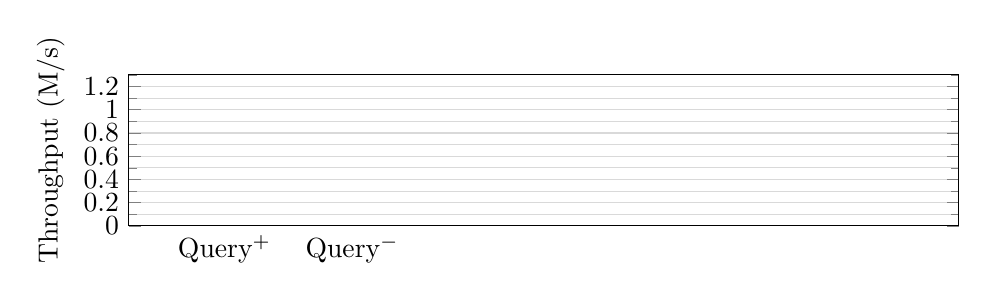
\begin{tikzpicture}
        \begin{axis}[
                width=\linewidth,
                height=3.5cm,
                ylabel={Throughput (M/s)},
                ybar,
                bar width=3pt,
                enlarge x limits=0.15,
                xtick={0,1,2},
                xticklabels={Insert, Query$^{+}$, Query$^{-}$},
                axis lines=box,
                tick align=inside,
                xtick style={draw=none},
                scaled ticks=true,
                tick label style={/pgf/number format/fixed,/pgf/number format/precision=1},
                ymajorgrids=true,
                yminorgrids=true,
                minor tick num=1,
                max space between ticks=35pt,
                try min ticks=5,
                grid style={gray!30},
                enlarge y limits={upper,value=0.3},
                ymin=0,
                nodes near coords,
                nodes near coords align={vertical},
                nodes near coords style={/pgf/number format/fixed, /pgf/number format/precision=0, font=\tiny, rotate=90, anchor=west, yshift=0.5pt, xshift=0.3pt},
                legend entries = {\htthree, \htfour, \htfive, \htsix, \htone, \httwo},
                legend cell align = left,
                legend style={draw=none, legend columns=3, /tikz/every even column/.append style={column sep=1cm}},
                legend to name={L1-sized-table-legend-3column},
                unbounded coords=discard,
                filter discard warning=false,
            ]

            \addSmallTablePlots

        \end{axis}
    \end{tikzpicture}

    \caption{Throughput on small table (2047 entries) across operations.}\label{fig:small_table_throughput}
\end{figure}
